
%\documentclass[./main.tex(path of main file)]{subfiles}
\documentclass[10pt]{article}
\usepackage{amsmath}
\DeclareMathOperator*{\argmin}{arg\,min} % thin space, limits underneath in displays
\DeclareMathOperator*{\argmax}{arg\,max} % thin space, limits underneath in displays
\newtheorem{thm}{Theorem}
\usepackage{amssymb}
\usepackage{amsfonts}
\usepackage{mathrsfs}
\usepackage{bm}
\usepackage{indentfirst}
\setlength{\parindent}{0em}
\usepackage[margin=1in]{geometry}
\usepackage{graphicx}
\usepackage{setspace}
\doublespacing
\usepackage[flushleft]{threeparttable}
\usepackage{booktabs,caption}
\usepackage{float}
\usepackage[sort,comma]{natbib}
\usepackage[hidelinks]{hyperref}
\usepackage{booktabs}
\usepackage{multirow}

\usepackage{import}
\usepackage{xifthen}
\usepackage{pdfpages}
\usepackage{transparent}
\usepackage{subfiles}
\usepackage{blindtext}
\usepackage{glossaries}
\usepackage{pdflscape}
\usepackage{adjustbox}
\usepackage{rotating}
\usepackage{eurosym,geometry,ulem,subcaption,caption,color,sectsty,comment,footmisc,pdflscape,array}

% Format definition list
\newenvironment{mylist}[1]%
  {\begin{list}{}{\settowidth{\labelwidth}{\textbf{#1}}
   \setlength{\leftmargin}{\labelwidth}
   \addtolength{\leftmargin}{\labelsep}
   \renewcommand{\makelabel}[1]{\textbf{\hfill##1}}}}%
  {\end{list}}



\newcommand{\incfig}[1]{%
\def\svgwidth{\columnwidth}
\import{./figures/}{#1.pdf_tex}
}




\title{}
\author{}
\date{}


\begin{document}
\maketitle

\tableofcontents
\newpage

\section{History of Macroeconomics}
\subsection{Phase 0: Panics of the 1800s and early 1900s}
\subsection{Phase 1: Measuring Macroeconomic Activity (1930s to Early 1950s)}
During the Great Depression, Maynard Keynes  published the General Theory of Employment, Interest,
and Money in 1936.
The basic tenet of the ``Keynesian view" was that various ``rigidities" plague market transactions
and lead to potentially long-lasting disequilibrium outcomes. The clearest way to understand
Keynesianism was that nominal wages and/or prices may not adjust quickly enough to clear quantity
supplied and quantity demanded. Hence Keynesian logic demands that the government should and is able
to aid the economy.

In order to do so, there needed to be some US-wide measures of the performance of markets; until
the Great Depression, there were none. The system of GDP accounting that we more or less still
continue to use began during the Great Depression. The concepts and measurements of aggregate GDP
and aggregate consumption and aggregate investment that we now take for granted in the typical
basic macroeconomics-class GDP accounting equation were essentially invented during the Depression.

By the mid-1940s, economists had collected and tabulated about 15 years of quarterly data (roughly
60 time periods) on what now are considered ``standard macro measures" often used to judge that
society's standard of living. There are two basic findings. First, in the long-time horizon there
is a steady upward march of GDP (long-term trend). Second, there are many ups and downs along this 
long-run path, called business cycle.

Should there be one unified framework to consider both long-run growth and business cycle 
fluctuation of the economy? The answer to this question is no. Understanding, both empirically and
theoretically, the long-run growth component is often referred to as the branch of 
{\underline {economic growth}} or {\underline {economic development}}; understanding the short-run
fluctuations of the economy is almost universally referred to as the branch of 
{\underline {macroeconomics}}.

\subsection{Phase 2: Keynesian Macroeconometric Approach (Early 1950s to late-1970s)}
The end of WWII is often attributed to the powerful engineering and technology the US military
rapidly developed. This is also the period in which newly developed mainframe computers using punch
cards to process computations were being increasingly put to research use.

The mathematically and computationally based ideas crept into macroeconomic thinking. Not
uncoincidentally, much of the high-powered technology that aided military efforts was developed
at research universities at which top-notch economists were also housed.

Starting in the early 1950s, a heavy does of mathematics and statistical analytics using high-powered
mainframes quickly became the fashion of macroeconomics, first in academic circles and then,
by the early 1960s, in policy circles. A paramount goal for these emerging computable
statistical description of aggregate economic events--the Keynesian macroeconometic approach--was
to answer an important question hanging over macroeconomics: How can business cycle be 
``explained"?

Throughout the 1950s many Keynesian macroeconometric framework were developed around the world.
One prominent large-scale Keynesian macroeconometric frameworks that quickly took center stage
was the MIT/Penn/Federal Reserve Board model constructed by a consortium of researchers and policy
advisers at these three institutions.

Championing this effort was a group of three prominent economists from academe, all of whom would be future Nobel laureates—Paul Samuelson (Nobel recipient in 1970), James Tobin (Nobel recipient in 1981), and Robert Solow (Nobel recipient in 1987). Samuelson, Tobin, and Solow were not cloistered academics in the Ivory Tower. Each spent significant time in his career serving in various government positions that advised President John F. Kennedy and President Lyndon B. Johnson, including serving on the White House Council of Economic Advisers.

The Keynesian-inspired macroeconometrics models took the form
\begin{align*}
x_{1t}&= \alpha_0x_{2t} + \alpha_1x_{3t} + \alpha_2x_{4t} + \cdots\\
x_{2t}&= \alpha_3x_{1t} + \alpha_4x_{3t} + \alpha_5x_{4t} + \cdots\\
\cdots &\\
x_{136t}&= \alpha_{597}x_{1t} + \alpha_{598}x_{13t} + \alpha_{599}x_{69t} + \cdots,
\end{align*}
where $ \alpha $ describes the correlation observed in the real world between an economic 
variable on the RHS and the economic variable on the LHS.

The US economic growth was incredibly strong during the 1950s and 1960s, perhaps in part due to 
the ``great policy tips" provided by the estimated models (from Keynesian approach). It came to the
point where macroeconomic ups and downs started to be considered a solved problem.

This seemed to be true throughout the 1950s and 1960s--but it then turned out to be no longer
true in the stagflationary period of the 1970s and early 1980s. All of a sudden, the glory decades of macroeconomics of the 1950s and 1960s seemed to have collapsed. If macroeconomics were to remain an organized field of thought, scores of economists figured that the future of macro had to somehow depart from Keynesian macroeconometrics because there was something seemingly inconsistent with economic analysis in these frameworks.

Many researchers struggled to describe the essence of this inconsistency. Finally, in 1976, it was the economist Robert Lucas (future Nobel recipient in 1995) who simply and elegantly described the root of the issue. His (later named) {\underline {Lucas critique}} pointed out that the $ \alpha $
coefficients were essentially never seriously through of as being dependent on policy.
A much larger, much deeper issue arose from the Lucas critique, which is that Keynesian 
macroeconometic models are noto economic models, but rather only statistical descriptions
of economic outcomes.

There are alternative ways of ``defining" economics, but the theme that runs through them all is that
economics studies how individuals make informed choices given scarce resources. Do the $ \alpha $
terms capture these ideas? The answer was no. The macro profession was in disrepute by the late
1970s, on the verge of extinction.


\subsection{Phase 2.5: The Rise of Monetarism}
The rise of the monetarist school of thought bridged ``phase 2" and ``phase 3" of macroeconomic
though. Milton Friedman examined every downturn of the US economy since the mid-1800s and found that
they were all accompanied by either an outright decrease in the level of the supply of money or
a decrease in the growth rate of the supply of money.

Friedman's analysis led to the conclusion that the Federal Reserve should not have clamped down on the
nominal money supply in the early stages of the Depression.
Reagan found Friedman's descriptions clear. Friedman was to become an economic consultant
for Reagan's campaign for President in 1980.

Reagan won in a landslide against Jimmy Carter's re-election campaign, and Paul Volcker essentially
built directly on the monetarist idea, by clamping down tightly on the issuance of new nominal
money to bring down the inflation in the 1980s.

In terms of the proper  reach of macroeconomic policy and how prescriptive policy should be,
monetarism (sometimes known by the name ``quantity theory of money") ideologically bridged
the decline of the Keynesian macroeocnometrics phase in the 1970s with the emergence of the 
microeconomic-based approach of modern macroeconomics of the late 1970s and 1980s.


\subsection{Phase 3: Modern Macroeconomic Framework (late 1970s to Present)}
Modern macroeconomics begins by explicitly studying the microeconomic principles of 
utility maximization, profit maximization, and market clearing (micro-foundation). This 
modern macroeconomic approach quickly captured the attention of the profession through the 1980s for
two reasons. First, it actually begins with microeconomic principles. Second, it was in the early 
1980s that desktop computing started to become widespread. The new breed of modern macroeconomic
frameworks could thus be computed directly in one's office, rather than needing to reserve time for
use of costly mainframe machines.

Theories: 
\begin{itemize}
\item The real business cycle theory (RBC): consumption-leisure model, consumption-savings model, ...
\item The New Keynesian theory, which resuscitates Keynes's ideas of ``stickiness" in nominal
		prices, but in modern general-equilibrium macro form.
\end{itemize}


\begin{figure}[H]
\center{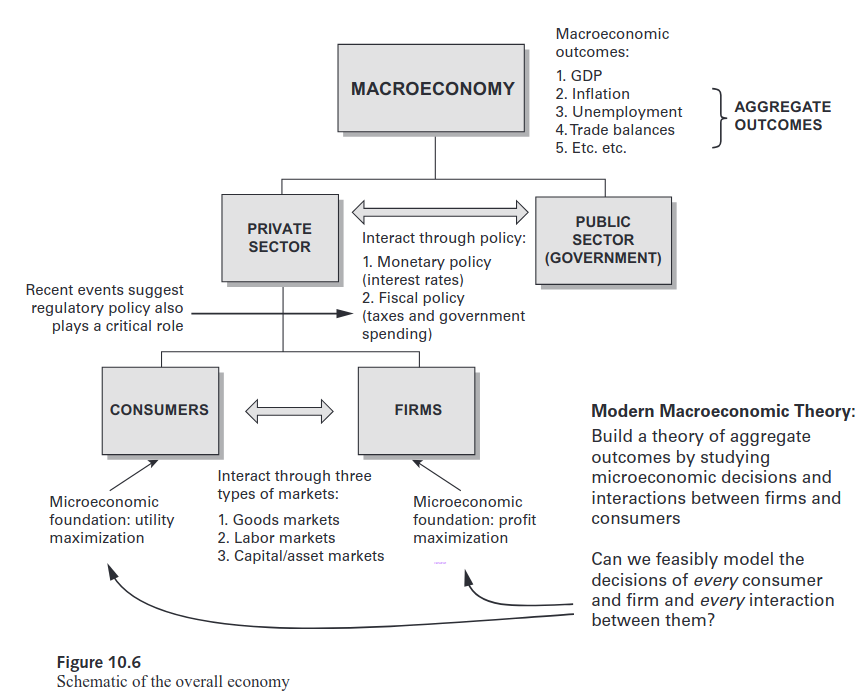
\includegraphics[width = 0.8\textwidth]  {figures/scheme_of_overall_economy.png}}
\label{fig:}
\end{figure}


\subsubsection{Supply-Side Economics}
\subsubsection{The Phillips Curve (PC)}

{\textbf {Nominal Wage Rigidity and the Short-Run PC}}:\\
With a perfectly competitive labor market, in equilibrium, cyclical unemployment is zero
(unemployment rate is equal to the natural rate of unemployment). Suppose there is a negative 
demand shock that shifts the aggregate demand to the left (price level drops),
labor demand then shifts to the left. With a perfectly competitive labor market,
wage rate decreases from $ w^{*} $ to $ w^{new} $ to clear the market (cyclical unemployment is still zero). Thus it would
seem that it is impossible for us to generate a negative relationship between inflation and
unemployment wherein cyclical unemployment never changes.


\begin{figure}[H]
\center{
\includegraphics[width = 0.8\textwidth]  {figures/wage_rigidity.png}}
\label{fig:}
\end{figure}




However, there is ample reason to believe that the labor market is far from perfectly competitive.
The strongest  evidence is that wages tend to move very slowly over time, even when other 
macroeconomic events would tend to suggest sharp movement in wages. 

Now suppose that there are some features of the labor market that prevent the wage from adjusting
immediately to match demand with supply. Given a negative demand shock (price decreases), 
labor demand shifts to the left but the wage rate remains stuck at $ w^{*} $ (known as 
wage rigidity or sticky wage). At the wage rate $ w^{*} $, quantity demanded for labor is less than 
quantity supplied of labor, and it brings cyclical unemployment to positive. This negative
relationship between the  inflation rate and the unemployment rate is captured by the 
(short-run) Phillips Curve.



{\textbf {Long-run PC}}:\\
Supposing that contracts that specify wages in advance are the primary source of wage rigidity, then
if aggregate demand continues to slump for a protracted period, we would expect the new
round of labor contracts negotiated when the original labor contracts expire to feature lower wages.
Continuing with our example from figure 12.4, new rounds of wage negotiation yield the lower
nominal wage $ w^{new} $, and it brings the cyclical unemployment to zero, i.e., even though
inflation stays low, unemployment rate will eventually gravitate back to its natural rate in
the long run. And this leads to a {\underline {vertical long-run Phillips Curve}}.

\begin{figure}[H]
\center{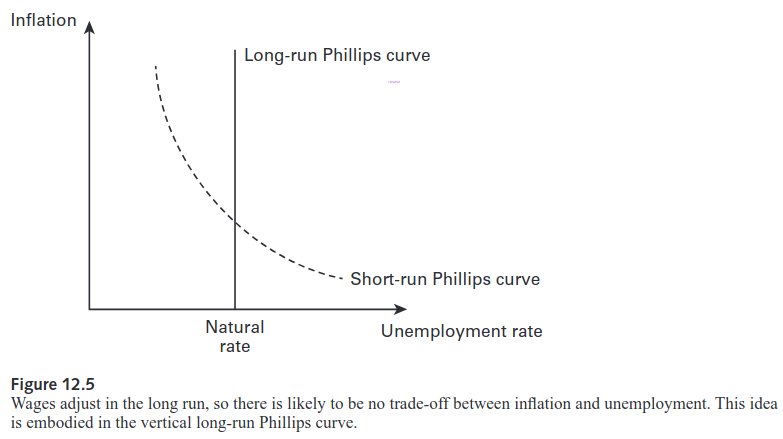
\includegraphics[width = 0.8\textwidth]  {figures/SR_and_LR_Phillips_Curve.png}}
\label{fig:}
\end{figure}



\subsubsection{Real Business Cycle Theory}
The two current leading views of business cycles are real business cycle (RBC) theory and New Keynesian economics. Each of these schools of thought has a rich history marked by frequent vigorous debate between them.

RBC theory views periodic expansions and recessions as natural, indeed efficient, responses of the economy to the ups and downs of the state of “technology” of the economy.1 As such, recessions are not dire events for the economy, but rather natural slowdowns that are preceded by an expansion and that will again be followed by future expansions. In terms familiar from microeconomics, pure RBC theory maintains that the aggregate economy operates perfectly competitively on both the demand side and the supply side.2 An important implication of RBC theory therefore is that the government has no role to play in the macroeconomy—that is, neither fiscal policy nor monetary policy can be used to improve the macroeconomic condition.

New Keynesian economics adopts the point of view that there are fundamental market failures in the aggregate economy that render business cycle fluctuations inefficient, specifically periods of lower than potential GDP.3 The important implication of this point of view is that the government may indeed have a role to play in improving macroeconomic conditions.

For the most part, RBC theory has held much less sway among policymakers than has New Keynesian theory. Among theoretical macroeconomists, however, RBC theory is very well-known and well-understood and even provides the foundations for some of New Keynesian theory.1 

Although there are a number of ways in which RBC theory differs from New Keynesian theory, we will focus on two differences.
\begin{itemize}
\item 
		The most important difference by far is that RBC theory eschews (avoid) the idea of sticky prices, while New Keynesian theory embraces it. RBC theory views prices as fully flexible.
    Even more precisely, RBC theory supposes that perfect competition in all markets is a good starting point for analyzing the macroeconomy. 
\item 
		Second, RBC theory does not view exogenous shifts of consumption demand as a good description of data but rather “shifts in supply” as the predominant reason for macroeconomic fluctuations.
\end{itemize}


{\textbf {Measure of Supply Shock}}
Consider the aggregate production function, $ A \cdot f(k, n) $, where $ A $ capture the 
technology improvement, called the Total Factor Productivity (TFP). This parameter is usually
identified with the Solow residual. This way of measuring technology has the virtue that it does not
require taking a stand on what constitute ``technology"--that is, it does not require identifying
the state of technology of an economy with, say, the number of computers it uses or with the number
of PhDs it employs, etc.

The most commonly-used production function in RBC theory is the Cobb-Douglass production function
\begin{equation*}
f(k,n) = k ^{\alpha} n^{1 - \alpha},
\end{equation*}
in which the parameter $ \alpha $ measures the percentage of total GDP that goes toward paying for
the costs of capital used in production. More common terminology is that $ \alpha $ is capital's
share of output and $ 1 - \alpha $ is labor's share of output. Empirical evidence shows that
for the US $ \alpha $ is about 0.33.

The total output (GDP) is determined by $ y = A \cdot f(k,n) = A \cdot k ^{\alpha} n^{1 - \alpha}$.
We observe $ y, k, n $ from the data, and assuming $ \alpha = \frac{1}{3} $, so we can calculate
$ A $.

The unexplained variation in the technology parameter $ A $ should be viewed as {\textbf {supply shocks}}.
In the influential study that effectively launched the RBC school of thought, Kydland and Prescott
(1982) found that fluctuations in the Solow residual accounted for well over half of fluctuations
in GDP, leading them to conclude that a theory of business cycle could be build with technology
as its centerpiece.


{\textbf {How Does the Technology Shock Work?}}
Assumptions
\begin{itemize}
\item Perfect competition
\item HHs owns capital and labor
\item Labor tax rate is always zero
\end{itemize}

Now suppose there is a temporary increase in $ A $.
Then, MPK and MPL increase, i.e., for a profit-maximizing firm, demand for capital and labor 
increases (shifts outward) as below. Real wage and rental price of capital for that firm is constant (horizontal
line) because a single firm is a price-taker in perfect competitive market.

\begin{figure}[H]
\center{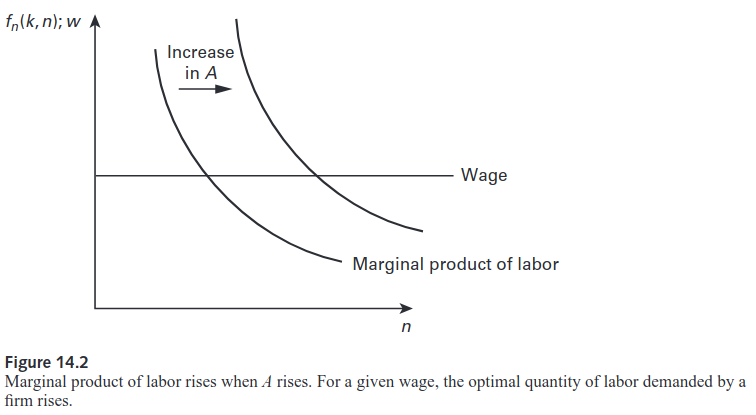
\includegraphics[width = 0.8\textwidth]  {figures/RBC_temp_A_up_MPL.png}}
\label{fig:}
\end{figure}

\begin{figure}[H]
\center{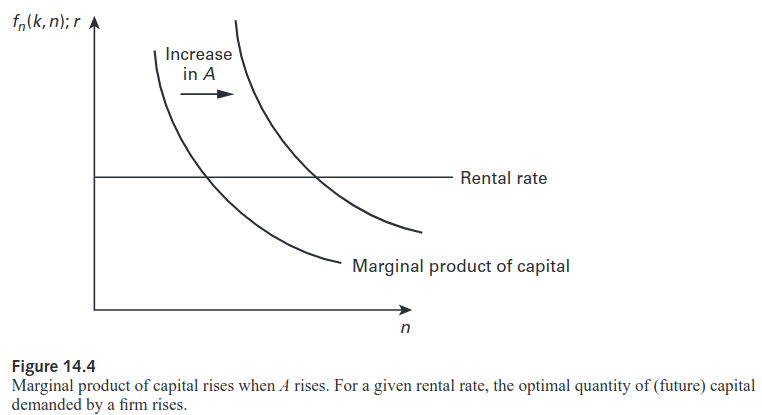
\includegraphics[width = 0.8\textwidth]  {figures/RBC_temp_A_up_MPK.png}}
\label{fig:}
\end{figure}

Now we look at the aggregate labor market and capital market. The right-shift in demand pushes
up the price of labor and capital and quantity.
The labor demand is derived from the consumption-leisure model. Note that here we assume that
the representative consumer is in the upward-sloping portion of the labor supply curve 
(backward-bended curve).

A rise in A rises the profit-maximizing quantity of (future) capital any given individual
firm desires. Thus {\textbf {the temporary increase in $ A $ led to an increase in both
future $ k $ and current $ n $ through its effects on factor prices. And therefore, total output
$ y $ unambiguously increases in both the current period as well as the future.}}

\begin{figure}[H]
\center{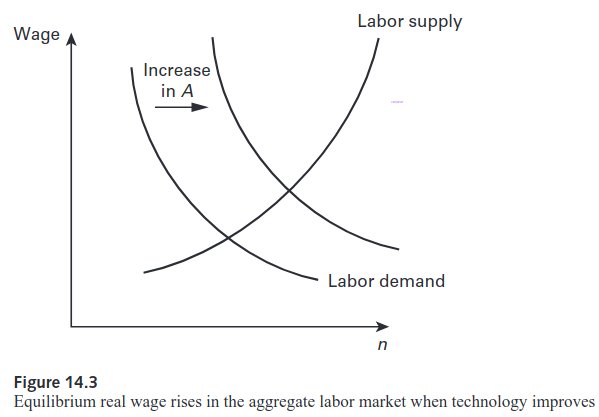
\includegraphics[width = 0.8\textwidth]  {figures/RBC_temp_A_up_labor_demand.png}}
\label{fig:}
\end{figure}


\begin{figure}[H]
\center{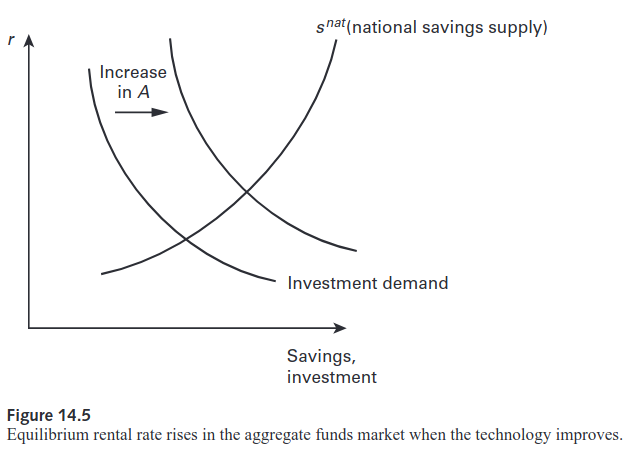
\includegraphics[width = 0.8\textwidth]  {figures/RBC_temp_A_up_investment_demand.png}}
\label{fig:}
\end{figure}

Now that we have traced out the aggregate effects, we next examine the representative consumer's
response along both the static consumption-leisure margin and the consumption-savings margin.

For consumption-leisure margin, as real wage rises, the budget constraint steepens as a result,
the new optimal choice of $ (c,l) $ in the current period features higher consumption and
less leisure (work longer).

For consumption-savings margin, an increase in current labor and future capital results in a 
higher income in both current and future income, i.e., both $ y_1 $ and $ y_2 $ increases in the
two-period model. Also, as real interest rate rise, the LBC becomes steeper.

\begin{figure}[H]
\center{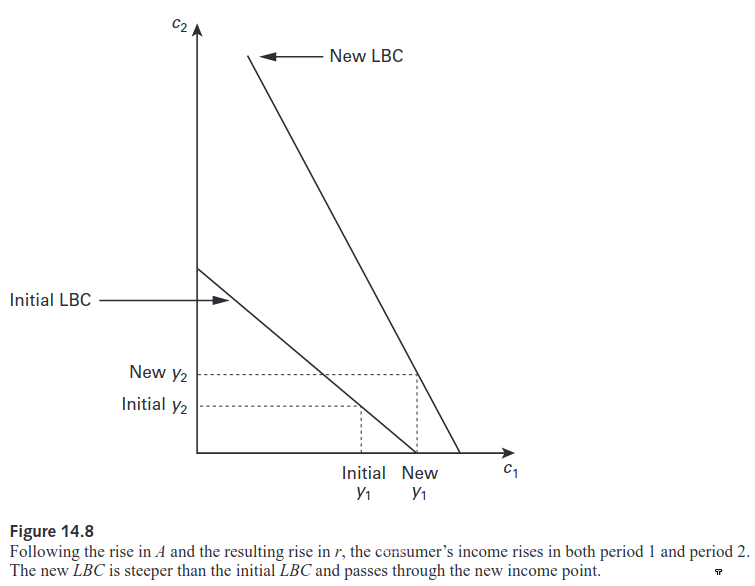
\includegraphics[width = 0.8\textwidth]  {figures/RBC_temp_A_up_new_LBC_consumption_savings.png}}
\label{fig:}
\end{figure}

As shown below, consumption in period 1 increases but does not rise by as much as income rises.
The consumer thus optimally spends only part of the gain in period-1 income and save the rest for
period 2. This illustrates the important principle of {\underline {consumption-smoothing}}.
Thus output rises in both period 1 and 2--in the parlance of the RBC literature, the temporary
(i.e., for only one period) technology shock leads to a persistent (i.e., for more than one-period)
change in output and consumption.


\begin{figure}[H]
\center{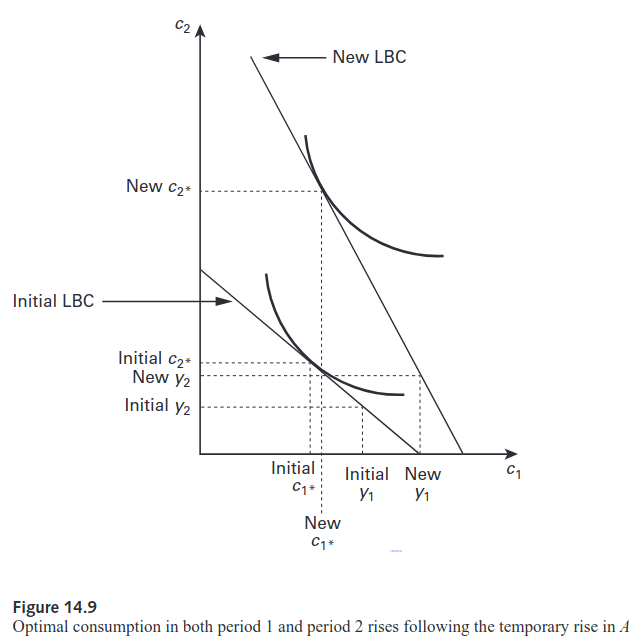
\includegraphics[width = 0.8\textwidth]  {figures/RBC_temp_A_up_new_optimal_choice_consumption_savings.png}}
\label{fig:}
\end{figure}








\subsubsection{New Keynesian Theory}
As we will see, microeconomic analysis is at the heart of New Keynesian theory. Unlike most of our
discussion of representative-agent macroeconomics, however, the focus of New Keynesian theory is not on the microeconomics of consumer behavior but rather on the microeconomics of firm behavior.
\\

{\textbf {Summary of Assumptions}}:\\
\begin{itemize}
\item 
		Instead of having just one consumption goods, now consumption is a function of a vast number
		of goods and services that are substitutable.
\item 
		Each of the $ N $ differentiated goods is assumed to be produced by a distinct monopolistically
		competitive firm.
\end{itemize}
%\\




{\textbf {Differentiated Goods and Consumption Aggregator}}:\\
In consumption-leisure and consumption-savings model, we assume there is only one object (i.e., 
``all stuff") that the consumer purchased in order to obtain utility. The use of a single good
is obviously a theoretical simplification. In reality, these goods are somewhat substitutable for 
each other, e.g., playing badminton vs. playing soccer.

If we believe that there are available a great many options for consumption, each of which is at
least a little different from every other option, then one way to reconcile our previous use of a 
single consumption good with this fact is to suppose that ``all stuff" is composed of these great
many differentiated goods. And this ``all stuff" consumption function can be written as
\begin{equation*}
c = c(c^{1}, c^{2}, \cdots, c^{N}),
\end{equation*}
where $ c^{i} $ denotes the type-$ i $ (or the $ i $th good), while we assume there are $ N $ 
different goods. This function is called the {\underline {consumption aggregator function}}.

In theoretical New Keynesian models, the function $ c(\cdot) $ is usually assumed to satisfy
the following two properties:
\begin{align*}
\frac{\partial c(\cdot ) }{\partial c^{i} } &> 0\\
\frac{\partial^{2} c(\cdot ) }{\partial (c^{i})^{2} } &< 0.
\end{align*}

These two conditions state that total consumption $ c $ is an increasing function of consumption
of type $ i $ and that total consumption $ c $ increases at an ever-decreasing rate as consumption
of type $ i $ increases. For example, the longer time you play badminton, the more total consumption
you enjoy--but the more and more you play, the less and less extra total consumption you gain.
One example of the consumption aggregator function is
\begin{equation*}
c(c^{i}, c^{2}, \cdots, c^{N}) = 
\left[ 
		(c^{1})^{\frac{1}{\varepsilon}} + (c^{2})^{\frac{1}{\varepsilon}} + ... + 
		(c^{N})^{\frac{1}{\varepsilon}}
\right] ^{\varepsilon},
\end{equation*}
where $ \varepsilon \ge 1 $. The value $ \varepsilon $ governs how substitutable, from the point of
view of the consumer, the different goods are for each other. With $ \varepsilon = 1 $, each
consumption good is just as good as any other, i.e., they are perfect substitutes for each other.
With $ \varepsilon > 1 $, however, goods are only imperfect substitutes for each other, 
meaning that they are differentiated to a degree depending on the exact value of $ \varepsilon $.
A basis for all of New Keynesian economics is the assumption that $ \varepsilon > 1 $.
\\



{\textbf {Monopolistically Competitive Firms}}:\\
Each of the $ N $ differentiated goods is assumed to be produced by a distinct monopolistically
competitive firm.
Recall that a fundamental feature of monopolistic competition is that goods are similar to each
other but not completely identical. Also, a firm that produces a differentiated good possesses
market power. And this market power manifests itself in the fact that the firm faces a 
downward-sloping demand curve (instead of a horizontal) and hence a marginal revenue curve that
lies strictly below its demand curve. This in turn implies that the firm's profit-maximizing
choice ($ MC = MR $ determines the quantity to produce, then together with the demand curve to 
determine the price) features price greater than marginal cost.

\begin{figure}[H]
\center{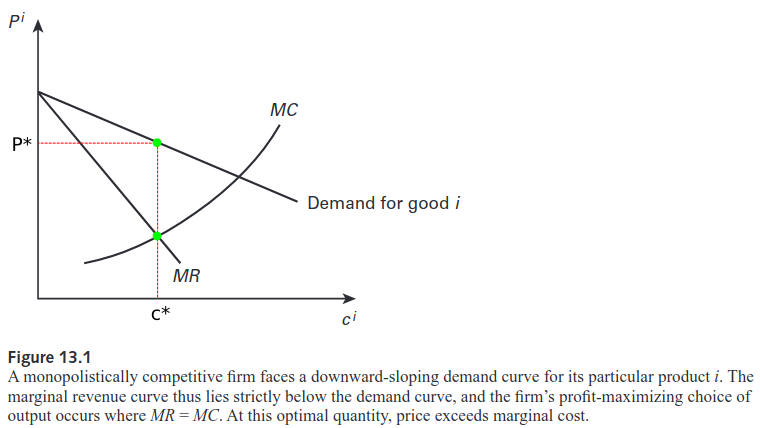
\includegraphics[width = 0.8\textwidth]  {figures/NK_monopolistic_competition_firm.png}}
\label{fig:}
\end{figure}

In an extreme case, $ \varepsilon = 1 $, firms do not have any market power (and thus face 
perfectly elastic demand curve as the case in the perfect competition, i.e., a horizontal line).
Thus setting $ \varepsilon = 1 $ is one way of shutting off the New Keynesian elements of a 
New Keynesian model.
\\


{\textbf {The Aggregate Price Level}}:\\
In the New Keynesian model, the aggregate price level $ P $ is a function of the price for each good,
\begin{equation*}
P = P(P^{1}, P^{2},..., P^{N}),
\end{equation*}
we call this function as price-level aggregator. The important feature of this function is that
$ P $ is strictly increasing in each of its arguments,
\begin{align*}
\frac{\partial P(\cdot ) }{\partial P^{1} } &> 0\\
\frac{\partial P(\cdot ) }{\partial P^{2} } &> 0.\\
\end{align*}
To draw an analogy with the consumer price index (CPI), if the price of any of the goods in the
CPI basket rises, the aggregate price level rises.
\\


{\textbf {Aggregate Consumption Demand}}:\\

The aggregate consumption demand is not the horizontal summation of each individual demand for
good type $ i $, since they are different goods, e.g., we cannot sum the demand for apple and the
demand for computer.
The consumption aggregator shows the relationship between aggregate consumption demand and the
demand for each of the differentiated goods. Recall that total consumption is an increasing function
of each type of differentiated good. This fact is all we need conclude that there is a positive
relationship between total consumption and consumption of each differentiated good.

The way to interpret the relationship depicted in Figure 13.2 is the following: when some event
(e.g., preference shocks and government policy shocks) shifts the consumption demand function,
the demand functions facing each firm also shift in the same direction. Because the individual
firm's demand functions shifts, the associated marginal revenue function shifts as well, implying
a new profit-maximizing choice of price and quantity for each individual firm.

You may notice that different from the RBC theory, New Keynesian theory argues that 
{\underline {``demand shocks"}},
coupled with the rest of the theoretical apparatus, are the predominant factor that causes 
macroeconomic fluctuations. In contrast, RBC theory argues that it is 
{\underline {``supply shocks"}}that
are the predominant source of macroeconomic fluctuations.


\begin{figure}[H]
\center{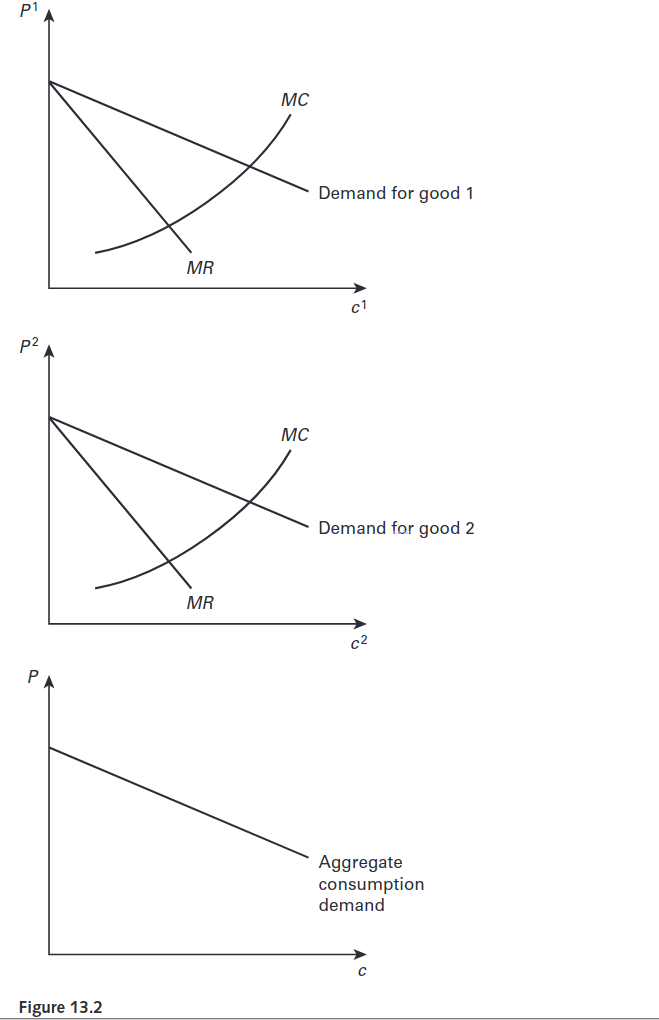
\includegraphics[width = 0.8\textwidth]  {figures/NK_aggregate_consumption_demand.png}}
\label{fig:}
\end{figure}
%\\


{\textbf {Staggered Price-Setting}}:\\
Consider the case in which the consumption demand function shifts outward for some reason. This event
in turn causes the demand functions, and hence the associated marginal revenue functions, facing
each individual firms to shift outward as well. Assuming the marginal cost functions do not shift,
event events in turn cause both quantity $ c^{i} $ and price $ P^{i} $ rise. Because the price
of each good rises, thee aggregate price level $ P $ rises as well.

However, suppose instead that only one of those firms can change its price at the time of the
event that shifts the aggregate consumption demand curve. Let's suppose that the rest of the firms 
have the ability to change price, while firm 1, in contrast, cannot change its price at all.

Figure 13.3 shows the events facing firm 1 following a rise in consumption demand.
Firm 1's demand function and MR function both shift outward. If Firm 1 were to change its price,
it would choose the price labeled ``optimal $ P^{1} $ if no price stickiness", and the quantity
would also rise. However, if firm 1 does not change its price and is forced to continue using the
initial optimal $ P_1 $, then its quantity produced will rise by even more (initial price together
with the new demand function), as can be read off the new demand function.


\begin{figure}[H]
\center{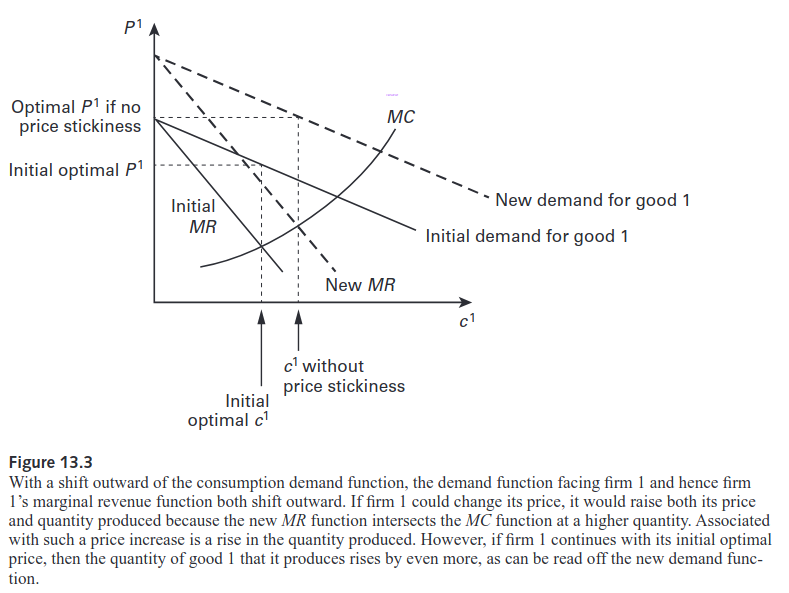
\includegraphics[width = 0.8\textwidth]  {figures/NK_price_stickiness.png}}
\label{fig:}
\end{figure}

%\\


{\textbf {Implications for Government Policy}}:\\
Now we consider how the macroeconomic effects of policy differ depending on whether firm 1 is able
to change its price. First, consider the case where all firms can adjust their price. When government
policy shifts the consumption demand outward, the aggregate price level $ P $ rises because the
price of each good rises.
Now, suppose that firm 1 does not have the ability to adjust the price while all other firms can do
so. All other firms raise their price in response to a positive demand shock. However, because
$ P^{1} $ does not change, the aggregate price level $ P $ does not rise by as mush as in the
case where firm 1 did change its price. Simultaneously overall consumption $ c $ rises by
more with firm 1's price held constant because $ c^{1} $ rises by more in this case.

In the preceding conclusion lie the important implications of New Keynesian theory for government
policy. In the presence of staggered price-setting, government policy that raises aggregate 
consumption demand {\underline {generates less inflation and a larger increase in production}}
than the same government policy in the absence of staggered price-setting.
Thus staggered price-setting gives economic policy makers leverage over real quantities in the
economy, more leverage than they would have if all firms could adjust prices simultaneously.
\\


{\textbf {Critique of New Keynesian Theory}}:\\
A long-standing criticism of the strand of New Keynesian theory that we have developed is the
assumption of staggered price-setting. We have offered no explanation why some firms cannot or does
not adjust its price while some others do change its price.

One common justification is the presence of asynchronous menu costs.
{\textbf {Menu costs are the costs incurred by a firm simply by the act of changing prices}}.
If different sectors of the economy experience menus costs of different magnitudes at different
times during the business cycle, then staggered price-setting may rise. While there is little
empirical evidence suggesting the magnitudes of these intangible menu cost, it is at least
a plausible story.

Strong empirical support for the New Keynesian view comes from data that suggest that government
policy, both fiscal and monetary, does have important short-run effects on output. Data generally
support the view that government policy is more effective that RBC theory predicts. This last
observation alone may be enough justification for studying New Keynesian theory.
\\











\section{Key concepts}
\subsection{Wealth vs. Income}
Income is a receipt of money by an individual during some period of time, such as labor income, 
interest income.
An individual's wealth is the level of assets (cash, checking accounts, savings accounts, stock, 
bonds, etc.) that an individual has in store. It can be negative if an individual is overdrawn
on his checking account or otherwise is in debt.

{\textbf {Example:}}:\\
If you have \$1000 in your savings accounts, then you have \$1000 in wealth.
If it generates \$30 interest in period 2, then your interest income is \$30.
If you earn a labor income of \$10000 in period 2, your total income is \$10030.

\subsection{First-Order Condition}
A first-order condition with respect to any particular variable mathematically describes how
a maximum is achieved by optimally setting/choosing that particular variable, taking as given the
setting/choices for all other variables.



\section{Dynamic Consumption-Savings Framework}
In this section, we will focus on the study of intertemporal (literally, ``across time")
choices of individuals.
We first ignore  leisure and labor altogether.

Consider a two-period model.

\subsection{Assumptions}
\begin{itemize}
\item 
		Each individual plans economic events for two time periods: present (period 1) and future 
		(period 2). There is no period 3! And every individual knows it!
		We will relax this assumption later.
\item 
		Individual has no control over his or her income. Each individual will receive labor income
		in each of the two periods. 
\item 
		Individual has to make a choice about consumption in each of the two periods.
\item
		Saving or borrowings (dissaving) are allowed during period 1.
\end{itemize}



\subsection{Model}
\subsubsection{Period-by-Period Budget Constraint}

\begin{align}
\text{ Period 1: }P_1c_1 + A_1 &= (1 + i)A_0 + Y_1 \label{eqn:t1_bc}\\
\text{ Period 2: }P_2c_2 + A_2 &= (1 + i)A_1 + Y_2 \label{eqn:t2_bc}
\end{align}
We must have $ A_2 = 0 $ as there is no period 3.



$ Y_1 $ is labor income received at the beginning of period 1. Each individual begins period 1
with some initial wealth (which may be negative), $ A_0 $. 
Each individual chooses consumption $ c_1 $ in period 1, each unit of which costs $ P_1 $ dollars.
He also decides how much wealth to carry into period 2, $ A_1 $. A negative $ A_1 $ means that 
the individual is in debt at the beginning of period 2. Nominal interest rate denotes as $ i $.

Private saving in a given time period is being defined as the difference between an individual's
total income and his total expenditures, consumption and taxes (we ignore taxes for now).
From the above, the total income is the sum of labor income and interest income,
\begin{equation*}
TotalIncome_1 = Y_1 + iA_0.
\end{equation*}
Thus saving in period 1 is
\begin{equation*}
S^{priv} = iA_0 + Y_1 - P_1c_1
\end{equation*}
If we rearrange equation \eqref{eqn:t1_bc},
\begin{equation*}
A_1 - A_0 = iA_0 + Y_1 - P_1c_1,
\end{equation*}
it says saving is the change in wealth during the course of a time period.

\subsubsection{Lifetime Budget Constraint}

$ A_1 $ appears in both equation \eqref{eqn:t1_bc} and \eqref{eqn:t2_bc}. Rearrange equation 
\eqref{eqn:t1_bc} by writting $ A_1 $ as a function of all other terms, then put it into 
equation \eqref{eqn:t2_bc}, we get.
\begin{equation}
P_1c_1 + \frac{P_2c_2}{1 + i} = Y_1 + \frac{Y_2}{(1 + i)} + (1 + i)A_0,
\end{equation}
which is the lifetime budget constraint (LBC).
If we write $ c_2 $ as a function of $ c_1 $, we get
\begin{equation}
c_2 =  - \frac{P_1(1 + i)}{P_2}c_1 + \frac{1 + i}{P_2}Y_1 + \frac{Y_2}{P_2} \label{eqn:lfb_nominal}
\end{equation}


\begin{figure}[H]
\center{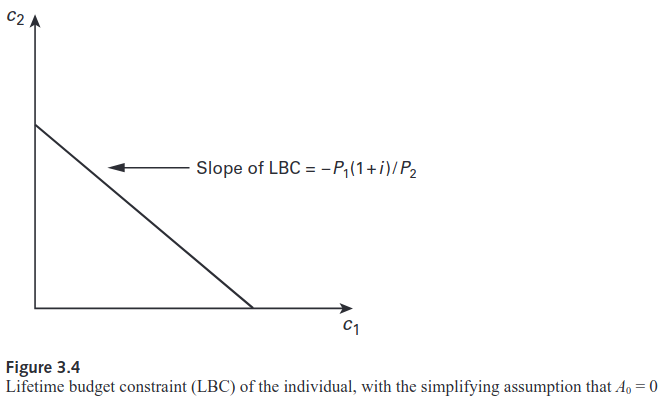
\includegraphics[width = 0.8\textwidth]  {figures/LBC_nominal_no_A0.png}}
\label{fig:}
\end{figure}




\subsubsection{Optimal Intertemporal Choice (Nominal Term)}
The optimal choice of consumption is the tangent point between the indifference curve and the LBC.
If we assume individuals consume more than they earn in period 1 ($ \frac{Y_1}{P_1} < c_1 $),
then they must consume less than what they would earn in period 2 ($ \frac{Y_2}{P_2} > c_2 $),
so they can pay the debt accumulated in period 1.
The figure below illustrate this situation.


\begin{figure}[H]
\center{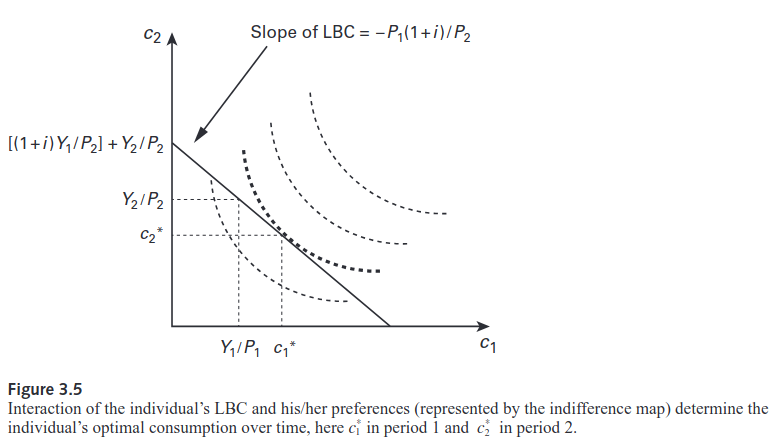
\includegraphics[width = 0.8\textwidth]  {figures/LBC_nominal_optimal_choice.png}}
\label{fig:}
\end{figure}


\subsubsection{Consumption-Savings Model in Real Units}


Recall the LBC in nominal terms,
\begin{equation}
P_1c_1 + \frac{P_2c_2}{1 + i} = Y_1 + \frac{Y_2}{(1 + i)} + (1 + i)A_0.
\end{equation}
To get the real unit, 
\begin{align}
c_1 + \frac{P_2}{P_1} \frac{c_2}{1 + i} &= \frac{Y_1}{P_1} + \frac{Y_2}{P_1(1 + i)} + 
(1 + i)\frac{A_0}{P_1}, \quad \text{ divide the nominal LBC by $ P_1 $ }\\
c_1 + \frac{P_2}{P_1} \frac{c_2}{1 + i} &= \frac{Y_1}{P_1} + 
\frac{P_2}{P_1}\frac{Y_2}{P_2(1 + i)} + 
(1 + i)\frac{A_0}{P_1}, \\
c_1 + c_2 \frac{1 + \pi_2}{1 + i}&= y_1 + y_2 \frac{1 + \pi_2}{1 + i} + (1 + i)\frac{A_0}{P_1},
\quad \text{ note, } \frac{P_2}{P_1} = 1 + \pi_2\\
c_1 + c_2 \frac{1 + \pi_2}{1 + i}&= y_1 + y_2 \frac{1 + \pi_2}{1 + i} + 
(1 + i)\frac{P_0}{P_1}\frac{A_0}{P_0},\\
c_1 + c_2 \frac{1 + \pi_2}{1 + i}&= y_1 + y_2 \frac{1 + \pi_2}{1 + i} + 
\frac{1 + i}{1 + \pi_1}a_0\\
c_1 + \frac{c_2}{1 + r}&= y_1 + \frac{y_2}{1 + r} + a_0(1 + r). \label{eqn:lbc_real_base}
\end{align}

If we write $ c_2 $ as a function of $ c_1 $ while assuming $ a_0 = 0 $ (for simplicity),
\begin{equation}
c_2 =  - (1 + r)c_1 + (1 + r)y_1 + y_2,
\end{equation}
the slope of the LBC now is $  - (1 + r) $.

\begin{figure}[H]
\center{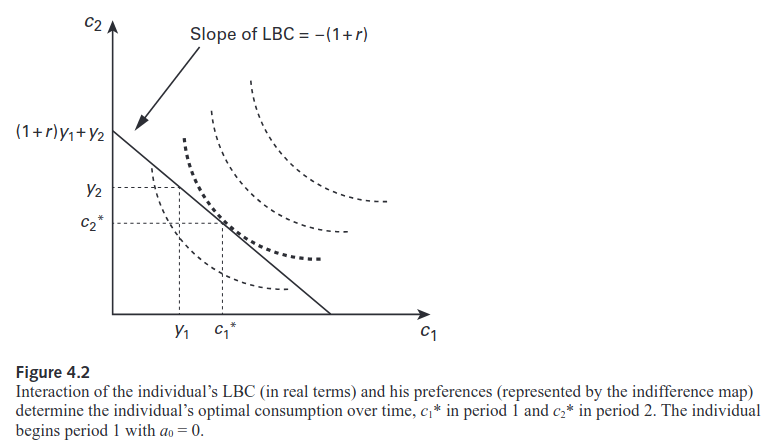
\includegraphics[width = 0.8\textwidth]  {figures/LBC_real_optimal_choice.png}}
\label{fig:}
\end{figure}

Note, {\textbf {the LBC must pass through $ (y_1,y_2) $}}.
Now let's consider what happens to this optimal choice if the real interest rate $ r $ rises, while
the labor income $ y_1 $ and $ y_2 $ both remain constant.
When $ r $ rises, the LBC becomes steeper (see below).


\begin{figure}[H]
\center{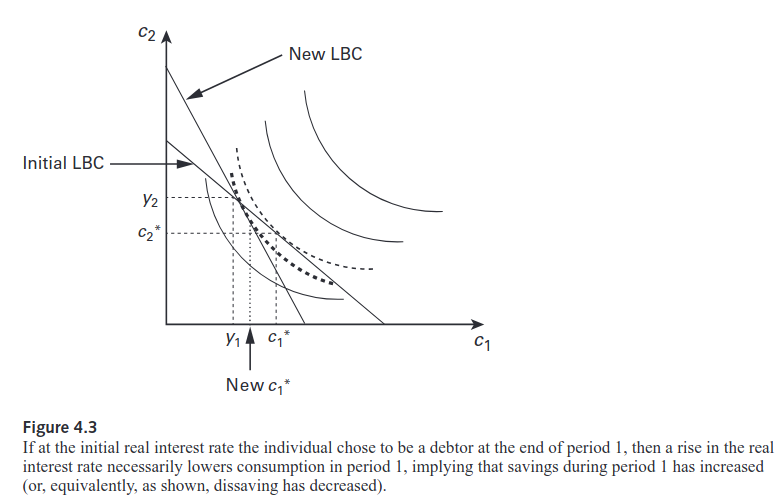
\includegraphics[width = 0.8\textwidth]  {figures/LBC_real_optimal_choice_r_rises.png}}
\label{fig:}
\end{figure}

Thus, by assume an individual is a debtor in period 1 ($ y_1 < c_1 $),
the models predicts a decrease in consumption, and thus an increase in savings, in period 1 when
real interest rate rises.


However, if we assume an individual is a saver in period 1 ($ y_1 > c_1 $), the model predicts that
a rise in $ r $ could either increase or decrease consumption. See the two figures below.

\begin{figure}[H]
\center{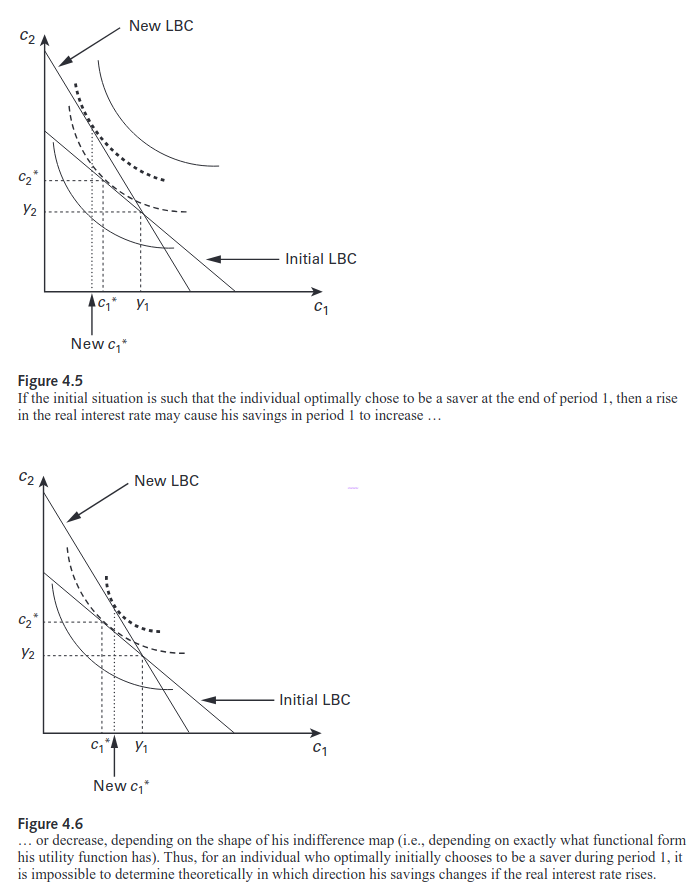
\includegraphics[width = 0.8\textwidth]  {figures/LBC_real_optimal_choice_r_rises_saver_period1.png}}
\label{fig:}
\end{figure}






\subsection{Results}
{\textbf {Real Interest Rate and Savings:}}
\begin{itemize}
\item 
		If an individual is initially a debtor (consumption is greater than income) at the end of period 
		1, then a rise in the real interest rate necessarily increases his savings during period 1.
\item 
		If an individual is initially a saver at the end of period 1, then a rise in the real interest
		rate may increase or decrease his savings during period 1.
\end{itemize}
{\textbf {Yet theory cannot guide use as to how private savings at the macroeconomic level
responds to a rise in the real interest rate!}}
Many empirical studies conclude that the real interest rate in fact has a {\underline {very weak 
effect}}, if any effect at all, on private savings behavior.

The studies that do show that real interest rates do influence savings almost always conclude that
a rise in the real interest rate leads to a rise in savings.




\subsection{Lagragian and FOC}

\subsubsection{Lifetime vs. Sequential Lagrange formulation}

In analyzing multi-period models using Lagrangians, it turns out we have two alternative and distinctly useful ways of proceeding: an approach we will refer to as a 
{\underline {lifetime Lagrange formulation}} and an approach we will refer to as a 
{\underline {sequential Lagrange formulation}}.

For a simple two-period model, the lifetime Lagrange formulation is essentially nothing more than a formal mathematical statement of the graphical analysis we have already conducted. It emphasizes, as the terminology suggests, that consumers can be viewed as making lifetime choices. The sequential Lagrange formulation emphasizes the unfolding of economic events and choices over time, rather than starting from an explicitly lifetime view. In the end, the sequential approach will bring us to exactly the same conclusion(s) as the lifetime approach; the sequential approach will thus seem like a more circuitous mode of analysis.\\

{\textbf {Why sequential Lagrange formulation}}:

We introduce the sequential Lagrangian approach, however, for two reasons. One reason is that when we soon extend things to an infinite-period model, in which graphical analysis becomes quite infeasible, the lifetime Lagrangian formulation (which, as just stated, is really just a mathematical formulation of analysis that can otherwise be carried out purely graphically) inherently becomes a bit less interesting. 

A second, and quite related, reason that sequential Lagrangian analysis is of interest is that it will allow us to explicitly track the dynamics of asset prices over time as macroeconomic events unfold over time.

\subsubsection{Lifetime Lagrangian Formulation}

Assume $ A_0 = 0 $,
\begin{equation}
u(c_1,c_2) + \lambda \left[ 
		Y_1 + \frac{Y_2}{1 + i} - P_1c_1 - \frac{P_2c_2}{1 + i}
\right] 
\end{equation}
\noindent\fbox{%
\parbox{\textwidth}{%
A first-order condition with respect to any particular variable (think in terms of basic calculus here) mathematically describes how a maximum is achieved by optimally setting/choosing that particular variable, taking as given the settings/choices for all other variables.
}%
}\\

In terms of the economics of our model, the consumer is optimally choosing {\underline {both}}
$ c_1 $ and $ c_2 $ (in order to maximize utility), which requires computing FOCs of the 
Lagrangian with respect to both $ c_1 $ and $ c_2 $.
\begin{align*}
\frac{\partial u }{\partial c_1 } - \lambda P_1 &= 0, \quad \text{ FOC wrt to $ c_1 $ }\\
\frac{\partial u }{\partial c_2 } - \lambda \frac{P_2}{1 + i} &= 0, \quad \text{ FOC wrt to $ c_1 $ },
\end{align*}
From the first equation, $ \lambda = \frac{u_{c_1}}{P_1} $, plug it into the second equation, we
get
\begin{align}
\frac{u_{c_2}}{u_{c_1}}&= \frac{P_2}{P_1} \frac{1}{1 + i}\\
\frac{u_{c_2}}{u_{c_1}}&= \frac{1 + \pi_2}{1 + i}\\
\frac{u_{c_2}}{u_{c_1}}&= \frac{1}{1 + r}
\end{align}
It says, when the representative consumer is making his optimal intertemporal choices, he chooses
$ c_1 $ and $ c_2 $ in such a way as to {\textbf {equate his MRS between period-1 consumption
and period-2 consumption to the real interest rate.}}


\subsubsection{Sequential Lagrangian Formulation}

In terms of constraints, in the sequential formulation we will impose all the period-by-period budget constraints, rather  than the LBC.
A review of basic mathematics (see the mathematical appendix at the end of the book) reminds us that it is straightforward to extend the Lagrangian method to handle optimization problems with multiple constraints. All we need to do, once we have identified the appropriate constraints, is associate distinct Lagrange multipliers with each constraint and then proceed as usual.

By assuming $ A_0 = A_2 = 0 $, the lagrangian is the following,
\begin{equation}
		u(c_1,c_2) + \lambda_1[Y_1 - P_1c_1 - A_1] + \lambda_2[Y_2 + (1 + i)A_1 - P_2c_2].
\end{equation}
Note, $ \lambda_1 $ and $ \lambda_2 $ are distinct multipliers, which has nothing to do with each 
other.

{\textbf {FOCs in period 1}}:

Note, in period 1, consumers choose $ c_1 $ and $ A_1 $ to maximize the utility, and therefore
we differentiate the lagrangian wrt $ c_1 $ and $ A_1 $, and get
\begin{align*}
\frac{\partial u }{\partial c_1 } - \lambda_1P_1 &= 0, \quad \text{ wrt } c_1\\
 - \lambda_1 + \lambda_2(1 + i)&= 0, \quad \text{ wrt }c_2
\end{align*}

{\textbf {FOCs in period 2}}:
We are supposed to differentiate wrt $ c_2 $ and $ A_2 $, since $ A_2 = 0 $, we only differentiate
the lagrangian wrt $ c_2 $,
\begin{equation*}
\frac{\partial u }{\partial c_2 }  - \lambda_2P_2 = 0
\end{equation*}

Combine the three FOCs, we get
\begin{align}
\frac{u_{c_1}}{u_{c_2}} &= \frac{(1 + i)P_1}{P_2}\\
&= 1 + r,
\end{align}
which is the same as what we got using the LBC.




\subsection{Solving for Numerical Choice}
We cannot solve for the numerical value of $ c_1 $ and $ c_2 $ using only the consumption--savings
optimality condition
\begin{equation}
\frac{u_{c_1}}{u_{c_2}} = (1 + r), \label{eqn:consumption_saving_condition}
\end{equation}
even when we know the form of the utility function. For example, if we assume, for simplicity, the
a log utility function, 
\begin{equation*}
u(c_1,c_2) = \ln c_1 + \ln c_2,
\end{equation*}
equation \eqref{eqn:consumption_saving_condition} becomes
\begin{equation*}
\frac{c_2}{c_1} = 1 + r.
\end{equation*}
However, we cannot solve for $ c_1 $ and $ c_2 $.
We need to use both the optimality condition and the budget constraint,
\begin{align*}
\frac{u_{c_1}}{u_{c_2}} &= (1 + r), \\
P_1c_1 + \frac{P_2c_2}{1 + i}&= Y_1 + \frac{Y_2}{1 + i}.
\end{align*}

{\textbf {Example (case1):}}

Suppose that the lifetime utility function is log utility. And also assume that $ P_1 = P_2 = 1 $,
$ A_0 = 0 $ and $ r = 0.1 $.

Further, assume $ Y_1 = 2, Y_2 = 11 $,
then the optimal consumption in period 1 and 2 would be
\begin{equation*}
c_1^{*} = 6, c_2^{*} = 6.6.
\end{equation*}


{\textbf {Example (case2):}}
Now if we assume this consumer earn more in period 1, $ Y_1 = 7, Y_2 = 5.5 $, the optimal consumption
is still
\begin{equation*}
c_1^{*} = 6, c_2^{*} = 6.6.
\end{equation*}


\noindent\fbox{%
\parbox{\textwidth}{%
{\underline {Clearly, the lifetime path of optimal consumption is the same,}} despite the large
difference between the case 1 lifetime income path ($ Y_1 = 2, Y_2 = 11 $) 
and the case 2 lifetime income path ($ Y_1 = 7, Y_2 = 5.5 $).

This example demonstrates the two different facets of {\underline {consumption smoothing}}.
\begin{itemize}
\item Individuals prefer their consumption across time to not vary very much, (6 and 6.6 are close).
		This result arises due to strictly increasing and strictly concave lifetime utility.
\item Despite the two very different income scenarios in the example, optimal $ c_1 $ and $ c_2 $
		are identical. This is due to the ability of the individual to borrow as much as he or she
		wants during period 1.

		If we force the consumer not to borrow in period 1, the case 1 consumption outcomes would be
		quite different: we would have $ c_1 = 2 $ and $ c_2 = 11 $ as the credit-constrained optimal
		choices.
\end{itemize}
}%
}\\


\section{Intertemporal Fiscal Policy (Ricardian vs. Non-Ricardian policy)}
Think about this question: whether government spending and taxes affect real interest rates.

The intersection of the upward-sloping savings curve and the downward-sloping investment curve
determines the equilibrium real interest rate in the economy. National savings is defined as
the sum of private and government savings,
\begin{equation*}
S^{national} = S^{private} + S^{government}.
\end{equation*}


\subsection{Ricardian Equivalence}

Government savings, in many cases, does not typically depend on market real interest rates.
Many politically related issues affect government spending and taxation, which in turn directly
affect government savings, regardless of what market interest rates might be. Political economy
issues are outside the scope of our analysis.

Recall that private savings does depend on the market real interest rate, through its effect on 
the slope of the consumer's lifetime budget constraint (private savings is an increasing function
of the real interest rate). Government spending, though, is {\underline {much less}} reliant on
market real interest rates because spending and taxation legislation can largely reflect other
concerns.


Given a lump-sum tax, the government LBC is
\begin{equation}
g_1 + \frac{g_2}{1 + r} = t_1 + \frac{t_2}{1 + r}, \label{eqn:gov_LBC}
\end{equation}
where $ g $ and $ t $ refer to government spending and taxes respectively.
Consumer LBC is
\begin{equation}
c_1 + \frac{c_2}{1 + r} = (y_1 - t_{1}) + \frac{y_2 - t_2}{1 + r}. \label{eqn:consumer_LBC}
\end{equation}
Combine consumer's and government's LBC, 
\begin{equation}
c_1 + \frac{c_2}{1 + r} = (y_1 - g_1) + \frac{y_2 - g_2}{1 + r} \label{eqn:gov_con_LBC}
\end{equation}

National saving is
\begin{align}
S_1^{national} &= S_1^{private} + S_1^{government}\\
&= y_1 - t_1 - c_1 + t_1 - g_1\\
&= y_1 - c_1 - g_1 \label{eqn:national_savins}
\end{align}


From equation \eqref{eqn:gov_LBC}, the path for government spending ($ g_1 $ and $ g_2 $) and
taxes ($ t_1 $ and $ t_2 $) must satisfy the government's LBC. Suppose that the government 
chooses to leave its spending plan unchanged but decides to lower $ t_1 $ for some reason, then it
must raise taxes in period 2 ($ t_2 $) since the government's present value of lifetime spending
is unchanged,
\begin{equation}
\Delta t_2 =  - (1 + r) \Delta t_1 \label{eqn:timing_of_taxes}
\end{equation}


The question we are interested in is 
{\textbf {whether this decrease in taxes in period 1 affects national savings in period 1}}.
From equation \eqref{eqn:national_savins}, we need to determine how, if at all, consumption
$ c_1 $ changes due to the change in the timing of taxes.

From equation \eqref{eqn:consumer_LBC}, the only way that the change in the timing of taxes would 
affect the optimal consumption choice of the individual is if the consumer's LBC is affected.
Looking at the RHS of equation \eqref{eqn:consumer_LBC}, suppose $ t_1 $ changes by $ \Delta t_1 $,
\begin{align*}
		[y_1 - (t_1 + \Delta t_1)] + \frac{[y_2 - (t_2 + \Delta t_2)]}{1 + r}
		&= [y_1 - t_1 - \Delta t_1] + \frac{[y_2 - (t_2 - (1 + r) \Delta t_1)]}{1 + r}\\
		&= (y_1 - t_1) + \frac{y_2 - t_2}{1 + r} - \Delta t_1 + \frac{(1 + r) \Delta t_1}{1 + r}\\
		&= (y_1 - t_1) + \frac{y_2 - t_2}{1 + r}.
\end{align*}
The lifetime resources the individual has available for consumption purchases is 
{\underline {NOT affected}} by the change in the timing of lump-sum taxes. Thus, the optimal
consumption choice is unchanged, and therefore national savings in period 1 is 
{\underline {unaffected by the change of the timing of lump-sum taxes}}. Thus real interest rate
is unchanged. This result is known as {\underline {Ricardian equivalence.}}

\noindent\fbox{%
\parbox{\textwidth}{%
Ricardian equivalence is the notion that holding fixed a path for government spending,
a change in the timing of taxes does not affect the equilibrium real interest rate because it
does not affect national savings.

In another word, the decrease in government savings (caused by a tax cut in period 1) is cover by an
increase in private savings (In order to pay more taxes in the future, fully rational consumers
will simply save the entire tax cut they receive today--which is what it means to say that private
savings increases by exactly the amount that government savings decreases), leaving national savings unaffected, which in turn leaves the 
equilibrium real interest rate unaffected.

Ricardian equivalence thus states that there is no connection between fiscal deficits and real 
interest rates.

}%
}\\


\subsection{Distortionary Taxes and The Failure of Ricardian Equivalence}

Instead of having a lump-sum tax, now we assume there is a sales tax $ \tau $. Then the consumer's
budget constraint becomes
\begin{align*}
(1 + \tau_1)c_1 + a_1 &= (1 + r)a_0 + y_1\\
(1 + \tau_2)c_2 + a_2 &= (1 + r)a_1 + y_2,
\end{align*}
and the LBC becomes
\begin{equation*}
(1 + \tau_1)c_1 + \frac{1 + \tau_2}{1 + r}c_{2} = y_1 + \frac{y_2}{1 + r},
\end{equation*}
and rearrange it to 
\begin{equation*}
c_2 =  - \frac{1 + \tau_1}{1 + \tau_2}(1 + r)c_1 + (1 + r)y_1 + y_2.
\end{equation*}

The slope of LBC is now clearly depends on the tax rates $ \tau_1 $ and $ \tau_2 $.
Holding fixed a path for government spending, suppose the government decides to lower the taxes rate
in period 1. To balance its LBC, the government must raise the tax rate in period 2.

In period 1, when $ \tau_1 $ decrease, the consumer LBC becomes flatter, and thus consumption in 
period 1 increases. It decreases the national saving in period 1 (supply shifts to the left), 
and therefore, real interest rate rises. {\underline {Ricardian equivalence does not hold}}.









\section{Infinite-Period Framework}
\subsection{Preferences}
The lifetime utility function is defined as the sum of all instantaneous utility function discounted
by the discount factor $ \beta $,
\begin{equation}
u(c_{t}) + \beta u(c_{t + 1}) + \beta^{2} u(c_{t + 2}) + \cdots =
\sum\limits_{s = 0} ^\infty 	\beta^{s}u(c_{t + s}).
\end{equation}

We use the discount factor $ \beta $ to represent the idea that utility further out in the future
is not as valuable as utility closer in time to the present moment. The discount factor $ \beta $
is between zero and one. 
\begin{itemize}
\item Consumers are perfectly patient if $ \beta = 1 $
\item Consumers are perfectly impatient if $ \beta = 0 $
\end{itemize}

The parameter $ \beta $ is meant to be a crude way of modeling the idea of {\underline {impatience}}.
All else equal, most of us would prefer to have $ x $ units of goods right this instant rather than
one year from now, and we would probably also prefer to have those $ x $ units one year from now
rather than two years from now. This is reflected by 
$ \beta < 1, \beta < \beta^{2}, \beta^{2} < \beta^{3}, \cdots $.


\subsection{Budget Constraint}
Suppose the assets that consumers buy and sell are ``shares in the stock market", and they can receive
dividends from holding stocks. Then our infinite-period model's period-$ t $ flow budget constraint
is 
\begin{equation}
P_{t}c_{t} + S_{t}a_{t} = S_{t}a_{t - 1}  + D_{t}a_{t - 1} + Y_{t},
\end{equation}
where $ S_{t} $ is the nominal price of stock, and $ D_{t} $ is a nominal dividend paid by each share.
Asset holding at the end of period $ t $ is $ a_{t} $.
Consumption and labor income in period $ t $ is $ c_{t} $ and $ Y_{t} $ respectively.


\subsection{Lagrangian}
The sequential Lagrangian becomes
\begin{align*}
u(c_{t}) &+ \beta u(c_{t + 1}) + \beta^{2} u(c_{t + 2}) + \beta^{2} u(c_{t + 3}) + \cdots\\
& + \lambda_{t}[Y_{t} + S_{t}a_{t - 1} + D_{t}a_{t - 1} - P_{t}c_{t} - S_{t}a_{t}]\\
& + \beta\lambda_{t + 1}[Y_{t + 1} + S_{t + 1}a_{t} + D_{t + 1}a_{t} - P_{t + 1}c_{t + 1} - S_{t + 1}a_{t + 1}]\\
& + \beta^{2}\lambda_{t + 2}[Y_{t + 2} + S_{t + 2}a_{t+1} + D_{t + 2}a_{t+1} - P_{t + 2}c_{t + 2} - S_{t + 2}a_{t + 2}]\\
& + \cdots,
\end{align*}

Note carefully that the $ t + 1 $ budget constraint in the Lagrangian is discounted by $ \beta $.
This is because {\underline {everything}} about period $ t + 1 $ is discounted when viewing from
the perspective of time $ t $, including income and expenditures.

{\textbf {FOC wrt $ c_{t} $ and $ a_{t} $}}:

\begin{align*}
u'(c_{t}) - \lambda_{t}P_{t}&= 0\\
 - \lambda_{t}S_{t} + \beta \lambda_{t + 1}(S_{t + 1} + D_{t + 1})&= 0.
\end{align*}

From the FOC on consumption in period $ t $, $ \lambda_{t} = \frac{u'(c_{t})}{P_{t}} $.
From the FOC on consumption in period $ t + 1 $, $ \lambda_{t + 1} = \frac{u'(c_{t + 1})}{P_{t + 1}} $.
Insert $ \lambda_{t} $ and $ \lambda_{t + 1} $ into the FOC on shares of stock, we have
\begin{equation}
\frac{u'(c_{t})S_{t}}{P_{t}} = \beta \frac{u'(c_{t + 1})(S_{t + 1} + D_{t + 1})}{P_{t + 1}}.
\label{eqn:FOC_on_stock}
\end{equation}
We can interpret the result in two ways: one is geared toward macroeconomic analysis, the other 
toward financial market analysis.

\subsubsection{Macroeconomic Analysis}
First, rewrite equation \eqref{eqn:FOC_on_stock} to highlight the intertemporal marginal rate of 
substitution,
\begin{equation*}
\frac{u'(c_{t})}{\beta u'(c_{t + 1})} = \frac{S_{t + 1} + D_{t + 1}}{S_{t}}
\frac{P_{t}}{P_{t + 1}}.
\end{equation*}
The LHS is the intertemporal MRS. The first part of the RHS, $ \frac{S_{t + 1} + D_{t + 1}}{S_{t}} $,
is the holding return of the asset $ a_{t} $.
It measures the gain (or loss) of holding the asset $ a_{t} $ from period $ t $ to $ t + 1 $.
The second part of the RHS is just $ 1 + \pi_{t + 1} $. And therefore, the RHS can be view as the
real rate of return, which works similar to the $ 1 + r $ in the consumption-saving model.
The reason $ (1 + r) $ does not appear explicitly is simply because of the assumption about the
available assets we have made here. If we assume there are assets in the environment that pay
a nominal interest rate, we will have our $ 1 + r $ on the RHS.
\subsubsection{Financial market Analysis}
Page 130

\subsection{Steady State}

We define the steady state of an economy as a situation in which 
{\underline {all real variables stop fluctuating over time}},
i.e., the value of them becomes constant.
The steady state of an economy is often referred to as the {\underline {long-run equilibrium}}
of an economy--think of it, as the ``average" or ``potential" performance of the economy.

To provide ourselves some more notation, in steady state, the level of consumption and real
interest rate is the following,
\begin{align*}
c_{t} = c_{t + 1} = c_{t + 2} = \cdots &=  \overline{c}\\
r_{t} = r_{t + 1} = r_{t + 2} = \cdots &=  \overline{r}.
\end{align*}

Consider the expression mentioned above,
\begin{equation*}
		\frac{u'(c_{t})}{\beta u'(c_{t + 1})} = 1 + r_{t}.
\end{equation*}
This expression is nothing more than the infinite-period model's consumption-savings optimality
condition. In a steady state the optimality condition can be expressed as
\begin{align*}
		\frac{u'( \overline{c})}{\beta u'( \overline{c})} &= 1 +  \overline{r}\\
		\frac{1}{\beta} &= 1 +  \overline{r},
\end{align*}
The expression, $ \frac{1}{\beta} = 1 +  \overline{r} $ is the long-run consumption-savings
optimality condition, captures an extremely critical idea embedded in virtually all of modern
macroeconomic theory and thus is at the root of a wide range of both academic and policy discussions
of macroeconomics.


It says that {\underline {the real interest rate}} of the economy is fundamentally {\underline {tied
to}} the degree of impatience of consumers in the economy. The theoretical upper end of $ \beta $
is $ \beta = 1 $; if $ \beta = 1 $, then the long-run real interest rate equals zero. That is,
if consumers are perfectly patient ($ \beta = 1 $), there is no net real return from savings.

Suppose instead that $ \beta = 0.95 $, meaning that consumers are somewhat impatient. The long-run
real interest rate in the economy is roughly $  \overline{r} = 0.0526 $. Now suppose that
$ \beta = 0.9 $, then $  \overline{r} = 0.11 $.


\subsection{Overlapping Two-Period Frameworks}
The infinite-period framework is simply an infinite sequence of overlapping two-period frameworks.
In period 1 ($ t = 1 $), consumers make decision on $ c_1 $ and $ c_2 $, the slope of the budget
constraint is $  - (1 + r_1) $. 
In period 2 ($ t = 2 $), consumers make decision on $ c_2 $ and $ c_3 $, the slope of the budget
constraint is $  - (1 + r_2) $. 

...

\begin{figure}[H]
\center{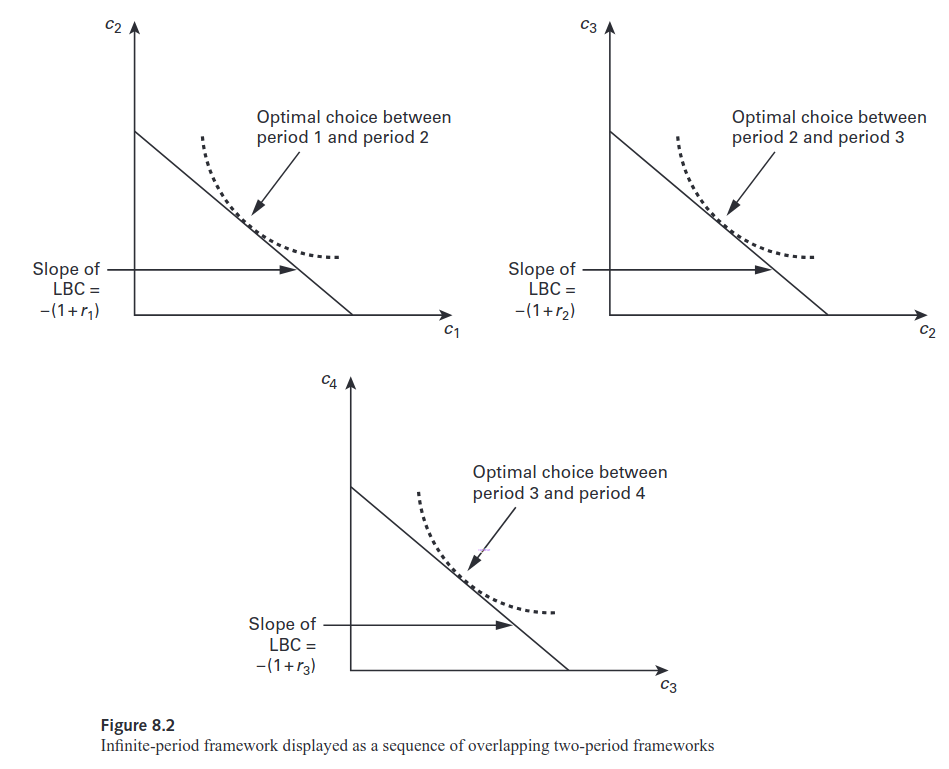
\includegraphics[width = 0.8\textwidth]  {figures/infinite_overlapping_two_periods_C-S_figure.png}}
\label{fig:}
\end{figure}



\section{Shocks}
The demand and supply relationships in the frameworks we have studied have been developed from 
microeconomic foundation, which are optimizations of some objective function subject to some
constraint function(s). The demand and supply relationships can {\underline {shift}} if either
or both the {\underline {objective function and constraint function(s)}} experience some
``changes".

In this section, we study sudden changes in an appropriate utility function if consumer analysis
is the focus, and in an appropriate profit function if  firm analysis is the focus.
These changes in foundations lead to precise shifts in the accompanying demand and/or supply curves.

The changes that we study here are termed {\underline {shocks}}. A shock is an unexplained
or unexplainable alteration in some basic element of an economic framework, which in turn
causes optimal choices to be affected.


\subsection{Production Shocks}
The introduction of a shock to the production function has the effect that for any given amount of
both capital and labor, total output depends on the level of the shock. Such a shock is most
commonly interpret as a ``technology shock."

The most usual way of introducing production function shocks is to suppose that it simply multiplies
the production function (parameter $ A $). If we set $ A = 1 $ always, then we recover the basic
two-period firm model we have studied. 

If $ A $ rises or falls, then the production function scales up or down. This technology shock
will be important in our upcoming discussion of {\underline {real business cycle theory}}.


\begin{figure}[H]
\center{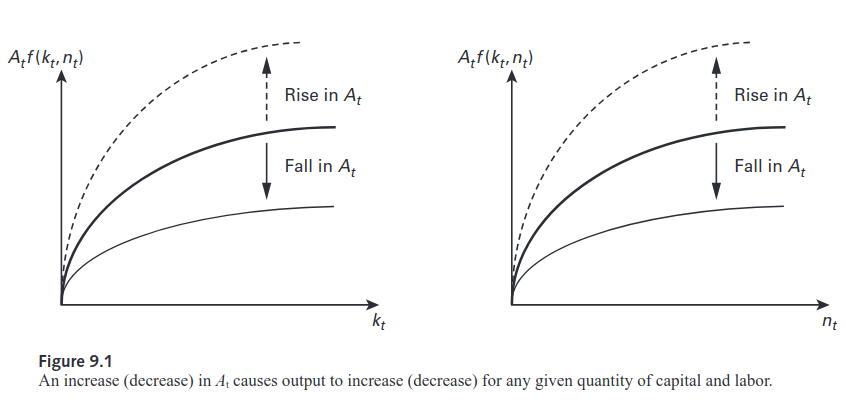
\includegraphics[width = 0.8\textwidth]  {figures/technology_shock.png}}
\label{fig:}
\end{figure}


\subsection{Preference Shocks}
Consider the utility function in consumption-leisure model, $ u(c,l) $, where $ c $ is consumption
and $ l $ is leisure. Now introduce a multiplier  for consumption, and therefore the utility
function becomes $ u(Bc, l) $,
where $ B $ is some given constant over which the individual has no control.
Suppose the new utility function takes the following form,
\begin{equation*}
u(Bc,l) = \sqrt {Bc} + \sqrt {l}.
\end{equation*}

Now suppose that all of a sudden $ B $ falls from 1 to 0.5 due to some unexplained event.
If we assume the optimal consumption given $ B = 1 $ is $ c^{*} = 10 $,
then the decrease in $ B $ causes consumption part drops from 
$ \sqrt {1  \times 10} \approx 3.16 $ to $ \sqrt {0.5  \times 10} \approx 2.23 $. This means
that each unit of consumption is now less valuable in utility terms. And therefore consumers
are willing to give up more units of consumption for a given increase in leisure. Thus the 
indifference curve of the individual would be steeper, as shown below

\begin{figure}[H]
\center{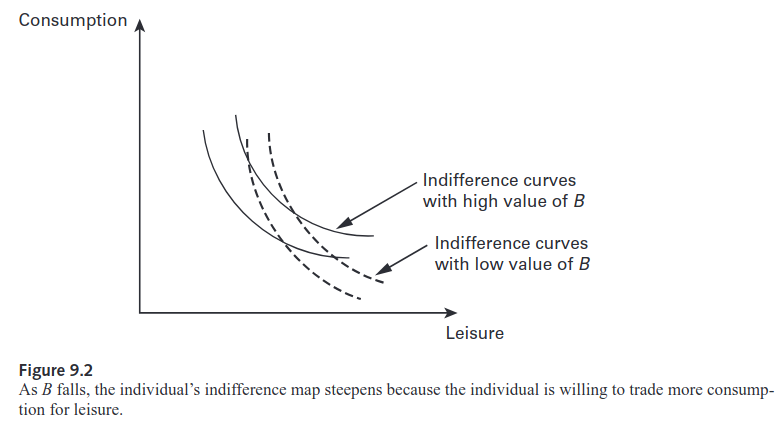
\includegraphics[width = 0.8\textwidth]  {figures/indifference_curve_preference_shock.png}}
\label{fig:}
\end{figure}

{\textbf {Results:}}

\begin{figure}[H]
\center{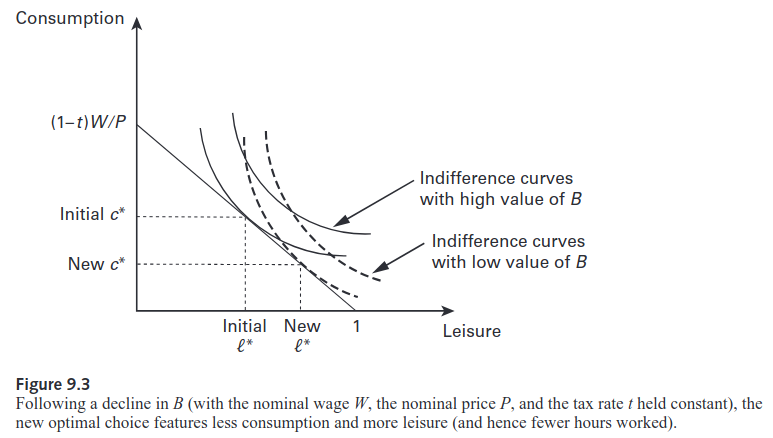
\includegraphics[width = 0.8\textwidth]  {figures/preference_shock_new_optimal_choice.png}}
\label{fig:}
\end{figure}



{\textbf {Given a lower $ B $, what's happening to the optimal consumption and leisure choice?}}:

With the wage rate $ W $, the price $ P $, and the labor tax rate $ t $ all held constant,
the new optimal choice features less consumption and more leisure--the latter implying that the
individual now works fewer hours
\\


{\textbf {Given a lower $ B $, what's happening to the labor supply?}}:

As consumers choose to work fewer hours, the entire labor supply curve must shift inward.
\\

{\textbf {Given a lower $ B $, what's happening to the consumption demand?}}:

The change in the optimal choice in figure 9.3 occurs with no change in the price P, i.e., such a 
reduction in consumption would occur for any given price $ P $. Thus, the consumption demand
function shifts inward.
\\

{\textbf {Given a lower $ B $, what's happening to the saving function?}}:
If we introduce this shock to the consumption-savings model, a decrease in consumption would cause the
aggregate savings function to shift.
\\



\section{General Equilibrium Macroeconomics}
General equilibrium occurs when all markets in the economy are simultaneously in equilibrium.
In contrast, partial equilibrium  occurs when one market in the economy achieves equilibrium, 
regardless of whether or not other markets have reached the point at which quantity supplied 
equates with quantity demanded.

Let's suppose that there are no distortionary taxes (lump-sum taxes only). 

{\textbf {Labor Market:}}\\
Let's take a look at the following pair of optimality conditions:
\begin{equation*}
\frac{u_{l}(c_{t}, l_{t})}{u_{c}(c_{t}, l_{t})} = w_{t}, \quad w_{t} = MPL_{t}
\end{equation*}
The expression on the left is the consumption-labor optimality condition, which is the 
{\underline {labor supply function}}.
The expression on the right is the firm's optimality condition regarding hiring, which is the
{\underline {labor demand function}}.
The equilibrium in the labor market occurs at the intersection of the supply and the demand,
\begin{equation*}
\frac{u_{l}(c_{t}, l_{t})}{u_{c}(c_{t}, l_{t})} = MPL_{t}.
\end{equation*}
The equilibrium occurs when the willingness of the consumer side of the economy to trade goods for 
leisure (which is the MRS between consumption and leisure) exactly equates with the extra (marginal)
productivity of an extra unit of time spent in labor.


{\textbf {Capital Market:}}\\
Consider the following pair of optimality condition:
\begin{equation*}
\frac{u'(c_{t})}{\beta u'(c_{t + 1})} = 1 + r_{t}, \quad r_{t} = MPK_{t}.
\end{equation*}
The expression on the left is the consumption-savings optimality condition, which yields the
private savings supply function.
The expression on the right is the firm's optimality condition regarding investing in new
physical capital for the future.
Put the demand  and supply together,
\begin{equation*}
\frac{u'(c_{t})}{\beta u'(c_{t + 1})} = 1 + MPK_{t}.
\end{equation*}


{\textbf {Goods Market}}:\\
Explain later.

Aggregate supply and aggregate demand.




\bibliographystyle{plainnat}
\bibliography{my_bib}

\end{document}

